%%
%% Template chap2.tex
%%

\chapter{Methods}
\label{cha:Methods}

In this chapter, we first gave an overview of the methods involved in this study. After that we explained how we collected our data and created labels. Then we introduced the principal model we used for image classification. On top of that, we investigated unsupervised learning methods to improve effectiveness and efficiency in the pre-training and prediction stage separately. Finally, the implementation details of our system were provided.

\section{Overview}
\label{sec:Overview}
In our study, we focused on a simple task of road scene understanding, which can be defined as to assign every part of a given image a label from one of the three classes, namely road, objects and sky. A widely used method is, for a single pixel, a patch consisting of its adjacent pixels will be used as the input for predicting the class of that pixel (Figure \ref{patchfig}), then the outputs from different parts of the image are organized together in a certain way to acquire the prediction result of the whole image. By adopting such approach we formalized our task mainly into a typical image classification problem.

\begin{figure}[h!]
\centering
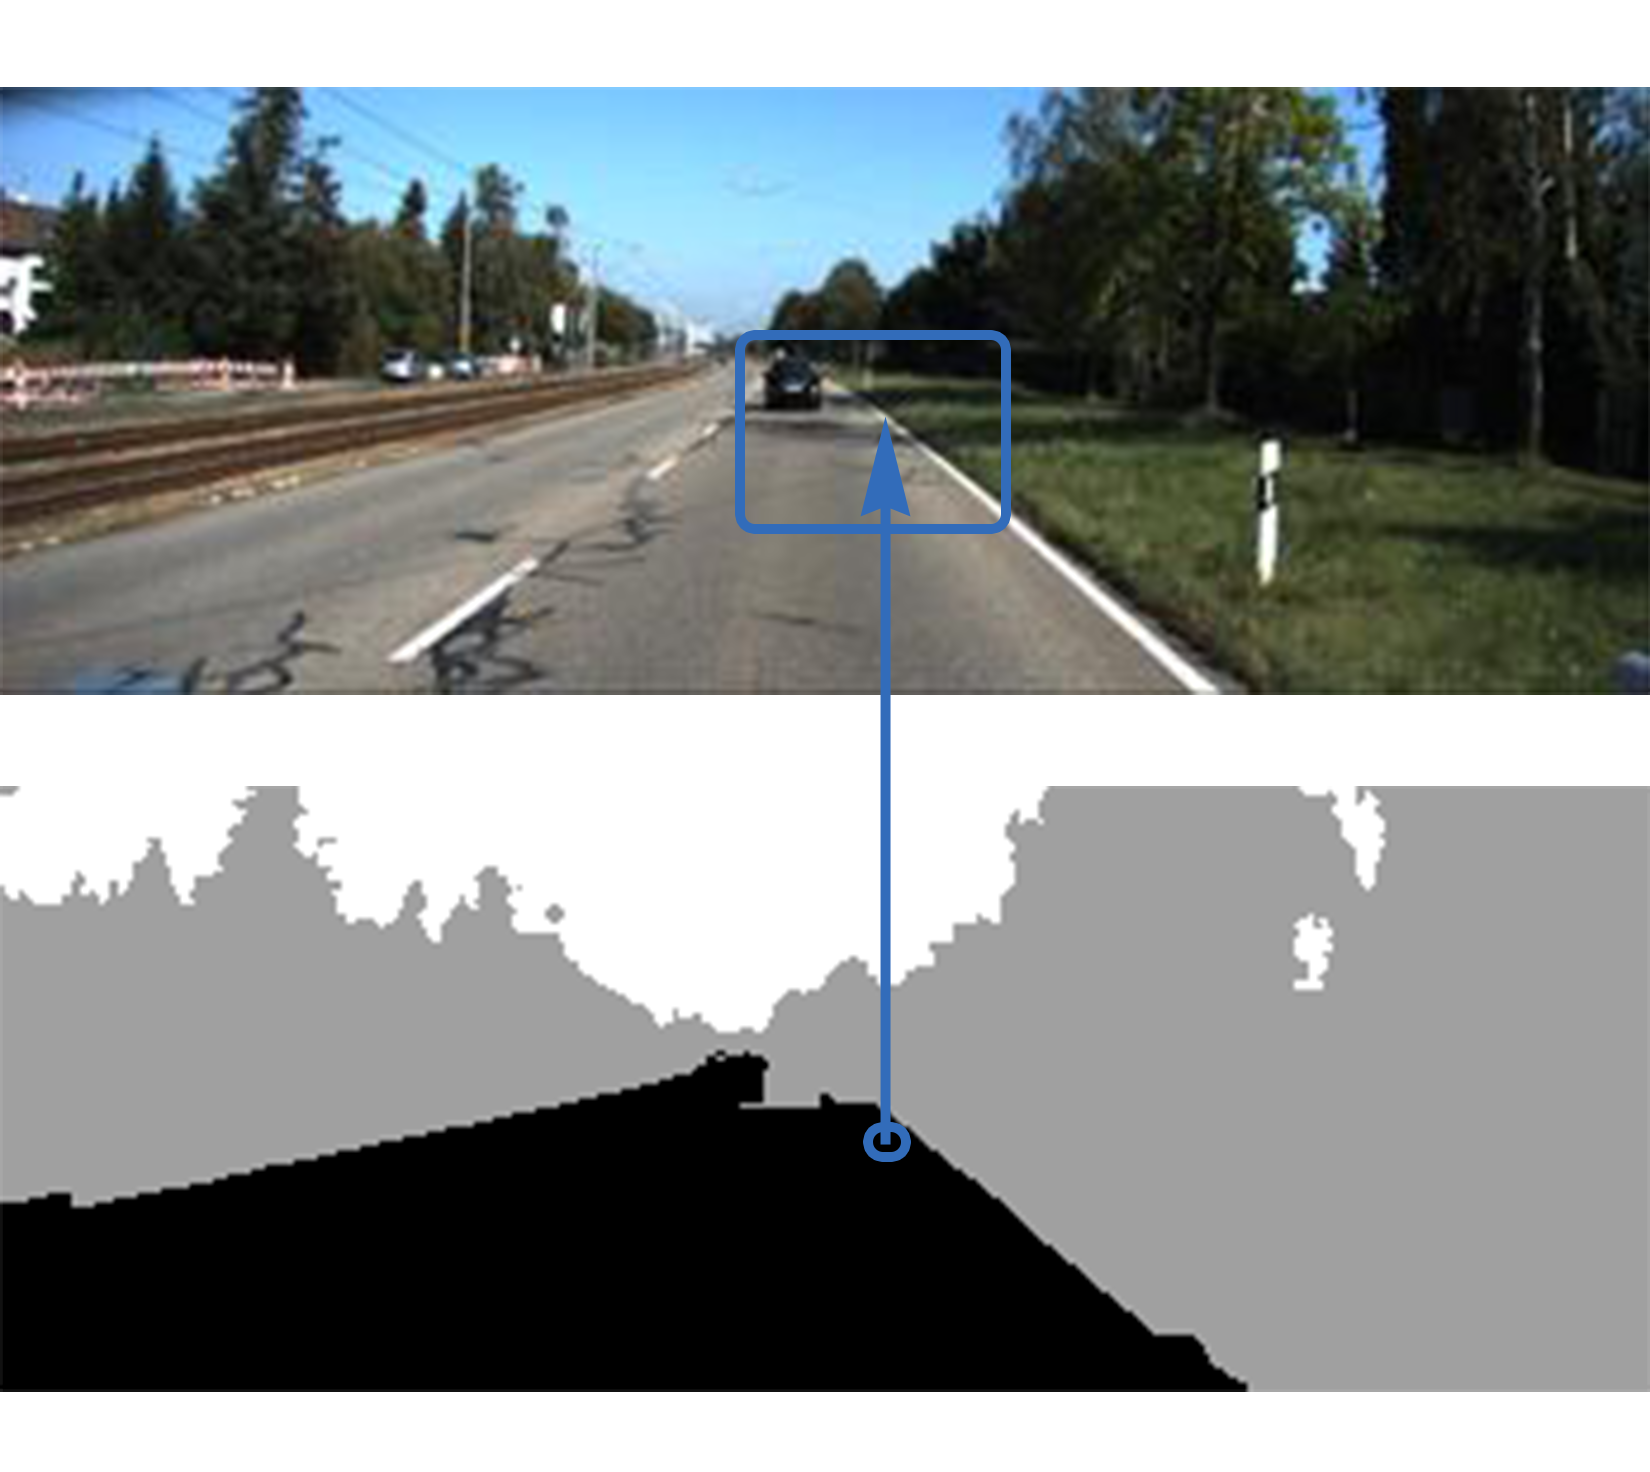
\includegraphics[width=0.7\linewidth]{pics/patch.png}
\caption{Only the area within the blue box in the original image (top) is extracted to be the input of predicting the label of the centering pixel (bottom).}
\label{patchfig}
\end{figure}

Therefore, we took Convolutional Neural Networks as a starting point, and applied various unsupervised learning approaches for the purpose of improving performance without losing generalizability. More specifically, we investigated unsupervised feature extraction methods including Principal Components Analysis and Convolutional Auto-Encoders. To further improve our performance in the prediction stage, several image segmentation algorithms were compared for super-pixel labeling. Finally, a method based on Markov Random Fields were experimented for reducing the noise of prediction output on a super-pixel level.

\section{Data}
\label{sec:Data}

\subsection{Data Source}
\label{sec:Data Source}
The KITTI data set~\cite{Geiger2013IJRR} is a comprehensive data set specially made for computer vision tasks about autonomous driving. We used the data provided in the KITTI ``road'' category, which consists of images taken by high-resolution color and grayscale video cameras equipped on a standard station wagon driving on main roads.

Because consecutive images taken within a short time slot are visually very similar, they are considered to be redundant in our study since we only take patches from a single image individually at a time. Therefore we selected only one out of five consecutive images from then ``road'' category, and partitioned the selected images into training and test sets.

\subsection{Label generation}
\label{sec:Label generation}
Apart from road scene images, we need their corresponding labels for training the classifier. Labels that suit our needs are not largely available. Since manually annotating labels is labour intensive and time consuming, we mostly used 3D reconstruction methods to generate labels for our data. 

Multiple view geometry based 3D reconstruction methods require more than one image from different perspectives of the same scenario, which is not applicable in our case. The ``photoPopup'' application is based on a trained classifier using handcrafted features, and is capable of roughly assigning each part of a single given images a label out of three categories namely, ground, sky, and vertical~\cite{hoiem2005automatic}. 

However this methods is inaccurate itself, and the ``ground'' category is not exactly what we defined as ``road''. For instance grasslands, railways and side walks are also expected to belong to the the ``ground'' category in the ``photoPopup'' application.  Therefore we manually discarded some labels of intolerable quality, and retain only about 50\% of the generated labels. After that, we had 264 labeled images in the training set, and 205 labeled images in the test set.

\subsection{Manual labels}
\label{sec:Manual labels}
In order to compare with and quantify the quality of generated labels. A subset of the images that contains 60 most visually different images (40 from the training set, 20 from the test set) were manually annotated by our collaborator Yi Liu. By comparing 60 manual labeled images against generated labels, we know the noise ratio of generated labels is approximately 12.74\%. A comparison of generated and manually annotated labels is shown in Figure \ref{genfig}.

\begin{figure}[h!]
\centering
\includegraphics[width=0.6\linewidth]{pics/gen.png}
\caption{Original image (top), generated labels (middle), manual labels (bottom). The areas within the red boxes of generated labels are considered as noise.}
\label{genfig}
\end{figure}

\section{Image Classification}
\label{sec:Image Classification}
Available machine learning methods are shown to have their own traits on different classification problems. For natural images and videos, adjacent pixels are believed to be highly correlated, which is associated with high redundancy if every pixel is treated as an independent dimension. Thus it is essential to take apply appropriate feature extraction methods in order to acquire good results and reduce algorithmic complexity.

For this reason many feature extraction methods are deliberately designed for image data, especially for images taken from man made objects. As discussed in Section \ref{sec:Handcrafted features}, these handcrafted feature extraction methods can excel in specific problems, but do not possess good generalizability.

From Section \ref{sec:Neural Networks} we know that neural networks are able to learn features implicitly given a redundant input. But since it employs a fully connected architecture, a large number of parameters may be involved, which is prone to overfitting and will increase the difficulty in training.

As described in Section \ref{sec:Convolutional Neural Networks}, convolutional neural networks can capture the correlation of adjacent values by taking discrete convolutions of receptive fields and kernel matrices, and is proven to be an effective approach for many image classification problems. Since weights are shared between receptive fields in different locations, it is able to extract local features and the number of parameters can be reduced substantially. By construct a deep architecture with pooling layers it is able to learn transition invariant and higher order features. Therefore convolutional neural networks are used as the main framework for learning and predicting the label of a given image patch. 

\section{Pre-training}
\subsection{Whitening}
\label{sec:Whitening}
From Section \ref{sec:Principal Component Analysis} we know that ZCA whitening can normalize the data to have zero mean and the same variance, while making the features less correlated. Such desirable properties has made it an important pre-processing step for many learning algorithms including convolutional neural networks. In particular, we did not perform dimensionality reduction and rotated the data to be as close as possible to the original data. By doing so we were able to preserve the intrinsic correlations between adjacent pixels, so that the pre-processed data would still be suitable as the input for convolutional neural networks.

\subsection{Unsupervised Feature Learning}
\label{sec:Unsupervised Feature Learning}

Since generated or manually annotated labels are insufficient either in  quality or quantity, to leverage the usability of unlabeled data is of great importance. Although PCA and auto-encoders are shown to be successful for general purpose feature extraction, they fail to capture the existing topology of the data by considering each input dimension independently. Convolutional auto-encoders offer a more sophisticated method for learning meaningful features from images in an unsupervised way. 

As was discussed in Section \ref{sec:Convolutional Auto-encoders}, convolutional auto-encoders can learn local and transition invariant features using similar architectural ideas as convolutional neural networks. But unlike convolutional neural networks, by using the input data as target output, convolutional auto-encoders can learn intrinsic features of the data itself instead of for some specific purpose. Therefore, features extracted by convolutional auto-encoders are believed to be more robust especially when training labels are noisy or insufficient. Moreover, higher order features can be obtained by training deep architectures in a layer-wise fashion~\cite{masci2011stacked}.

The reconstruction results also provide insights into the issue of how suitable the architecture is for our data. In general, as the complexity of the network architecture increases, the reconstruction error tends to go down. It normally will slowly approach to an asymptotic lower bound after the architectural complexity exceeds some certain point. Thus, the architectural complexity around that point is believed to be an suitable architecture for the data, which is neither too simple to cover important features nor too complex to manipulate.

Moreover, because the first layer kernel matrices are directly applied on input images, by visualizing the kernel matrices per feature map, we are able to interpret the conceptual meaning of some features, such as points, edges and colours. By visualizing the first layer kernels, we can gain a better understanding of indeed how convolutional neural networks and convolutional auto-encoders work.

Another significant benefit of convolutional auto-encoders is, the train results can be used to initialize a convolutional neural network of the same architecture by directly copying corresponding parameters. Optimizing highly non-convex objective functions arises in virtually all deep learning problems, such initialization can avoid numerous distinct local minima and yield a better result in many cases~\cite{masci2011stacked}. Furthermore, it also helps to reduce the number of iterations required in the training process than random initialization. 

\section{Prediction}
\label{sec:Prediction}

\subsection{Super-pixel labeling}
\label{sec:Super-pixel labeling}
So far we have investigated methods for predicting the label of a single pixel. The simplest approach for inferring all the labels of a given image would be to predict its labels pixel by pixel. Since an image often contains millions of pixels, such approach will be extremely inefficient. For instance, if a 32 by 32 patch is used for predicting one pixel, the amount of data we need to process for a 1024 by 1024 color image will then become $32\times32\times1024\times1024\times3$ pixels, which could be greater than one gigabyte.

A more efficient approach for inferring a whole image is by making use of super-pixels. More specifically, we first segment an image into super-pixels such that pixels within the same super-pixel are visually similar. After that, one representative are selected for each super-pixel. Then the inference result of the representative is shared among the pixels from the entire region covered by the super-pixel. The processing of arranging visually similar pixels into super-pixels is essentially another application of unsupervised learning called clustering, which is used to discover the hidden structure of the data.

As we discussed in Section \ref{sec:Image Segmentation}, the super-pixels generated using the graph-based image segmentation algorithm can be of arbitrary shapes (Figure \ref{gsuperfig}). Such irregular shaped super-pixels raise the difficulty of selecting sensible representatives. For instance, for a ring-shaped super-pixel, the mean or median of the coordinates of the points in that region in fact does not belong to the ring itself. Although there are techniques to select a medoid point, which is the member of a data set whose average dissimilarity to all the other points is minimal. Patches taken from the surrounding areas of such medoid points would still not be representative enough for such ring-shaped super-pixels.

The SLIC algorithm can generate super-pixels with an adjustable degree of spatial regularization. If a proper regularization parameter is chosen, we can obtain super-pixels whose shapes are regular enough to select good representatives from and are at the same time flexible enough to reflect the outline of an image (Figure \ref{slicfig}). For such regular shaped super-pixels, we can easily use their centroids as representatives. Moreover, the number of super-pixels generated by the SLIC algorithm can also be controlled approximately by another input parameter. This allows us to obtain a roughly fixed number of super-pixels regardless of the size of input image. In terms of time complexity, these two algorithms are both linear with regard to the size of the image.

\begin{figure}[h!]
\centering
\includegraphics[width=0.7\linewidth]{pics/slic.png}
\caption{Segmentation result of SLIC algorithm. Parameters are adjusted so that the shape of super-pixels are neither too fine or too coarse.}
\label{genfig}
\end{figure}

The benefits of this approach are, first, it can reduce the running time required for the inference steps substantially, if a fixed number of super-pixels is used, we can maintain the time complexity of preforming convolutional neural networks at a constant level. Second, since only centroids of super-pixels are used for inference, we managed to avoid the boundary points between super-pixels, where misclassifications are likely to happen. Third, since the same label in shared within a super-pixel that consists of visually similar images, the strong collation of adjacent pixels are captured in some sense.

\subsection{Super-pixel denoising}
\label{sec:Super-pixel denoising}
It can be expected from similar cases, our inference result can not reach a perfect accuracy. If it satisfies the case that a relatively small amount of misclassifications exist in our output, those misclassified super-pixels can be regarded as noise if a strong correlation of adjacent super-pixels is assumed. Then we can apply noise reduction methods on a super-pixel level in order to achieve a higher accuracy.

We focused on a graph denoising method using probabilistic graphical models. As described in Section \ref{sec:Markov Random Fields}, the MRF based graph denoising method tries to find a most likely state of the original graph according to a probabilistic distribution specified by some energy function (Equation \ref{energy}). Thus, the state of the highest probability will have the lowest energy.

We devised the energy function as follows. For the maximal cliques consisting of only an observed node and its connected latent node, the energy function is given by 
\begin{equation}
	E({C_{ol}}) = E({x_o},{x_l}) = 	
	\begin{cases}
    		0,& \text{if } x_o = x_l\\
    		1,              & \text{otherwise}
	\end{cases}
\end{equation}
where $x_o$ is the observed node and $x_l$ is the latent node. Therefore the clique will have zero energy if the observed node agree with the latent node, and vice versa. For the maximal cliques consisting of a set of mutually connected latent nodes, the energy function is given by 
\begin{equation}
	E({C_l}) =\frac{1}{Z} \sum\limits_{x_1\in C,x_2\in C}e(x_1,x_2)
\end{equation}
where $Z$ is a normalization factor depends on the size of the clique, and $e(x_1,x_2)$ is the energy between any pair of nodes in the form of
\begin{equation}
	e({x_1},{x_2}) = 	
	\begin{cases}
    		0,& \text{if } x_1 = x_2\\
    		1,& \text{if } x_1 \neq x_2\\
    		&\text{and one of them is of the ``objects'' state }\\
    		2,& \text{if } x_1 \neq x_2\\
    		&\text{and they are of the ``ground'' and ``sky'' state respectively}\\
	\end{cases}.
\end{equation}

According to the above energy function, if the ``ground'' and ``sky'' states exist in the same maximal clique, the clique will have a higher energy since these two states are not likely to appear closely together according to our prior knowledge. Apparently this is an empirical assignment, which should be tuned by more sophisticated methods. But this is beyond the scope of our study.

The total energy of the graph is given as 
\begin{equation}
	E({G}) =\alpha\sum\limits E({C_{ol}}) + \beta\sum\limits E({C_{l}}) 
\end{equation}
where $\alpha$ and $\beta$ are the parameters for controlling the extent of how much we want the latent node to be consistent with the observed nodes. Given the energy functions, we can use the iterated conditional modes algorithm to construct a less noisy graph.


\section{Implementation}
\label{sec:Implementation}
A software system was developed to explore the above described methods. We used Matlab as the main platform and integrated some C++ programs. The major components of the system include, label generation, convolutional neural networks, data pre-processing, convolutional auto-encoders, super-pixels and MRF denoising. The running time of the inference stage of our implementation is linear with regard to the size of the image, and only grows by a constant factor as the complexity of network architecture increases.

\subsection{Label generation}
For generating labels automatically, the ``photoPopup'' application (\url{http://dhoiem.cs.illinois.edu/projects/popup/}) was integrated to our system. Given an image, this application should be performed on the result of graph based image segmentation. An efficient implementation of graph based image segmentation using the disjoint sets data structure is available at \url{http://cs.brown.edu/~pff/segment/}.

\subsection{Classification}
Our implementation of convolutional neural networks was based on the DeepLearnToolbox library (\url{https://github.com/rasmusbergpalm/DeepLearnToolbox}) for Matlab, which applied stochastic gradient descent for network training~\cite{IMM2012-06284}. By the time our study was conducted, it only supported single channel input images. We did proper changes to make it compatible with multiple channel input data. We implemented ZCA whitening followed the guidelines on Stanford's UFLDL (\url{http://ufldl.stanford.edu/wiki/index.php/Whitening}).

\subsection{Convolutional auto-encoders library}
In terms of convolutional auto-encoders, to the best of our knowledge, there is no suitable libraries for our needs. We developed an open source library for convolutional auto-encoders named cae\_toolbox (\url{https://github.com/Dontloo/cae_toolbox}) according to~\cite{masci2011stacked}. The toolbox contained functions for training convolutional auto-encoders, visualizing training results and first layer kernels, and initializing convolutional neural networks which is compatible with the DeepLearnToolbox library.

The principal difficulty arose from evaluating the gradient information by error backpropagation. In addition, since discontinuous functions such as max pooling were engaged, it was crucial to ensure the correctness of the partial derivatives given in Equation \ref{caeeq}. 

To this end, we also evaluated the partial derivatives numerically. We first chose $\epsilon$ to be a small value (e.g., $10^{-6}$). For each parameter $\theta$, we computed the value of $E(\theta + \epsilon)$ and $E(\theta - \epsilon)$ while other parameters stayed unchanged. Then the partial derivative with regard to $\theta$ can be estimated in the form of 
\begin{equation}
	\frac{\partial E}{\partial \theta} = \frac{E(\theta + \epsilon)-E(\theta - \epsilon)}{2\epsilon}.
\end{equation}
By comparing with partial derivatives evaluated numerically, we have testified the correctness of our error backpropagation implementation.

\subsection{Prediction}
Two available implementations of the SLIC algorithm were compared in our study. The SLIC implementation for the VLFeat library (\url{http://www.vlfeat.org/overview/slic.html}) had the disadvantage of producing disconnected super-pixels, while another implementation from Image and Visual Representation Lab (IVRL) \url{http://ivrl.epfl.ch/research/superpixels} could produce more desirable results, hence was integrated into our system for the prediction stage. The optimization of the MRF energy function was implemented according to~\cite{kittler1984contextual}. 

%%% Local Variables: 
%%% mode: latex
%%% TeX-master: "thesis"
%%% End: 
